\documentclass[tikz,border=10pt]{standalone}
\usepackage{amsmath,amssymb}
\usetikzlibrary{calc,arrows.meta}

\begin{document}
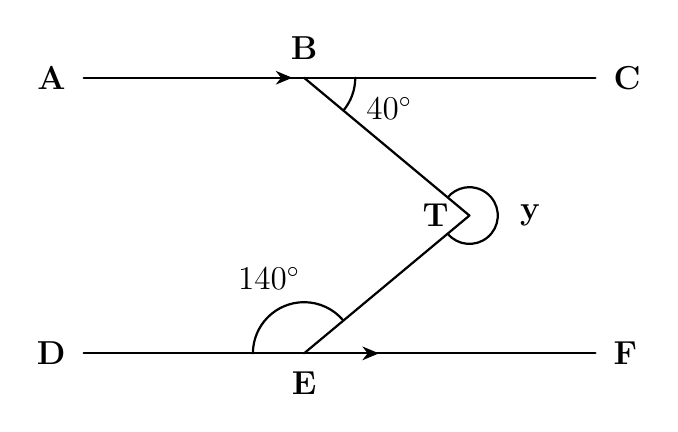
\begin{tikzpicture}[>=latex, line cap=round, line join=round]
  % Baseline coordinates
  \coordinate (A) at (0, 3.5);
  \coordinate (C) at (6.5, 3.5);
  \coordinate (D) at (0, 0);
  \coordinate (F) at (6.5, 0);

  % Vertex coordinates for exact 40-degree angles
  \coordinate (B) at (2.8, 3.5);
  \coordinate (E) at (2.8, 0);
  \coordinate (T) at (4.9, 1.75);

  % Parallel lines
  \draw[thick] (A) -- (C);
  \draw[thick] (D) -- (F);

  % Zigzag transversal segments
  \draw[thick] (B) -- (T) -- (E);

  % Parallel indicator arrows
  \draw[-{Stealth[length=6pt, width=5pt]}] (2.2, 3.5) -- (2.65, 3.5);
  \draw[-{Stealth[length=6pt, width=5pt]}] (3.3, 0) -- (3.75, 0);

  % Angle 40 deg at B
  \draw[thick] ($(B) + (0:0.65)$) arc (0:-39.8:0.65);
  \node at ($(B) + (-20:1.15)$) {\large $40^\circ$};

  % Angle 140 deg at E
  \draw[thick] ($(E) + (180:0.65)$) arc (180:39.8:0.65);
  \node at ($(E) + (115:1.05)$) {\large $140^\circ$};

  % Reflex angle y at T (sweeps from -140 deg around 0 to +140 deg)
  \draw[thick] ($(T) + (-140.2:0.36)$) arc (-140.2:140.2:0.36);
  \node[right=4pt] at ($(T) + (0:0.38)$) {\large $\mathbf{y}$};
  \node[left=4pt] at (T) {\large $\mathbf{T}$};

  % Vertex labels
  \node[left=3pt] at (A) {\large $\mathbf{A}$};
  \node[above=3pt] at (B) {\large $\mathbf{B}$};
  \node[right=3pt] at (C) {\large $\mathbf{C}$};
  \node[left=3pt] at (D) {\large $\mathbf{D}$};
  \node[below=3pt] at (E) {\large $\mathbf{E}$};
  \node[right=3pt] at (F) {\large $\mathbf{F}$};

\end{tikzpicture}
\end{document}
